\documentclass[../Kamil_Kowalewski_Main.tex]{subfiles}

\begin{document} {

    Z~powodu odwiecznej chęci rywalizacji między ludźmi na wielu płaszczyznach
    oraz coraz szybszego rozwoju technologii pojawiły się
    sporty samochodowe. Dzięki wybitnym konstruktorom, prężnym gałęziom przemysłu
    oraz genialnym naukowcom, powstawały coraz bardziej doskonałe pojazdy
    rozpalające jeszcze większą chęć rywalizacji w~bardzo zróżnicowanych
    warunkach. To właśnie dzięki tym pokoleniom ludzi możemy być teraz świadkami
    heroicznych zmagań kierowców.

    \section{Sporty samochodowe}
    \label{chapter2:wprowadzenie_sporty:sporty} {
        Sporty samochodowe są dyscypliną sportową skupiającą się współzawodnictwie,
        z~wykorzystaniem samochodów. Parametrem, poprzez który jest określany zwycięzca
        oraz kolejność innych uczestników jest zazwyczaj czas przejazdu określonego
        liczby okrążeń lub dojechanie do wyznaczonego punktu, który często jest trudny
        do osiągnięcia.

        Jako początek tej dyscypliny uznaje się rok 1894, kiedy został zorganizowany
        pierwszy rajd Paryż-Rouen. Dziesięć lat później czyli w~roku 1904 powstała FIA
        (fr. Fédération Internationale de l’Automobile) czyli międzynarodowa federacja
        sportów samochodowych. Cel z~jakim została stworzona to łączenie narodowych
        federacji odpowiedzialnych za sporty samochodowe.

        Ze względu na fakt, że w~wieku XX nastąpił bardzo duży rozwój nauki i~techniki
        same sporty samochodowe zaczęły bardzo się zmieniać i~specjalizować na
        kategorie zależnie od otoczenia, dystansu, reguł określających zarówno
        dozwolone i~niedozwolone zachowania jak i~sposób wyłaniania zwycięzcy. Stopień
        zaawansowania pojazdów i~ich części składowych takich jak silniki czy napędy
        znacznie wzrastały aby same zawody mogły się odbywać w~coraz to innych bardziej
        ciekawych warunkach wykraczających poza wyobrażenia osób biorących w~nich
        udział dwadzieścia lat wcześniej.

        \subsection{Podział sportów samochodowych}
        \label{chapter2:wprowadzenie_sporty:sporty:podzial} {
            Aktualnie po ponad 120 latach od pierwszego rajdu wspomnianego powyżej sporty
            samochodowe można podzielić na dwie główne kategorie:
            \begin{itemize}[noitemsep,topsep=2pt]
                \item Wyścigi na torach
                \item Rajdy na otwartej przestrzenii
            \end{itemize}

            \noindent Do wyścigów na torach można zaliczyć serie takie jak:
            \begin{itemize}[noitemsep,topsep=2pt]
                \item Formuły F1, F2, IndyCar, które odbywają się w~pojazdach
                jednomiejscowych
                \item Długodystansowe - ELMS (ang. European Le Mans Series),
                WEC (ang. World Endurance Championship)
                \item Turystyczne - DTM, TCR
                \item Amatorskie - imprezy jednodniowe (ang. Track day), przejazdy
                turystyczne na przykład na torze Nurburgring Nordschleife
            \end{itemize}

            \noindent Do rajdów na otwartej przestrzeni należą:
            \begin{itemize}[noitemsep,topsep=2pt]
                \item Rajdy terenowe np. Rajd Dakar
                \item Cykliczne rajdy organizowane przez FIA - WRC (ang. World Rally Championship),
                ERC (ang. European Rally Championship)
                \item Amatorskie - Imprezy jednodniowe (ang. Track day)
            \end{itemize}
        }

        \subsection{Najbardziej rozpoznawalne tory wyścigowe w Europie}
        \label{chapter2:wprowadzenie_sporty:sporty:tory} {
            W Europie jak i~na całym świecie od początku XX wieku powstało wiele
            torów wyścigowych oraz obiektów ogólnego użytku, które są wykorzystywane
            w~sportach samochodowych. W~Europie większość państw o~wysokim produkcie
            krajowym brutto PKB posiada tory wyścigowe, jedne mniejsze znane lokalnie
            oraz większe, na których odbywają się na przykład wyścigi Formuły 1. Wiele
            z~tych większych obiektów zasłynęło ze względu na to, że wymagają bardzo
            wysokich umiejętności od kierowców czy też bardzo ciekawą i~unikalną
            charakterystyką niespotykaną nigdzie indziej na świecie. Poniżej zostały
            przedstawione wybrane z~nich znajdujące się w~Europie oraz wybrane tory
            zlokalizowane w Polsce:
            \begin{itemize}[noitemsep,topsep=0pt]
                \item Niemcy
                \begin{itemize}[noitemsep,topsep=0pt]
                    \item Nurburgring Nordschleife
                    \item Nurburgring GP
                \end{itemize}

                \item Wielka Brytania
                \begin{itemize}[noitemsep,topsep=0pt]
                    \item Silverstone Circuit
                \end{itemize}

                \item Hiszpania
                \begin{itemize}[noitemsep,topsep=0pt]
                    \item Circuito Ascari
                \end{itemize}

                \item Belgia
                \begin{itemize}[noitemsep,topsep=0pt]
                    \item Circuit de Spa-Francorchamps (pot. Spa)
                \end{itemize}

                \item Węgry
                \begin{itemize}[noitemsep,topsep=0pt]
                    \item Hungaroring
                \end{itemize}

                \item Polska
                \begin{itemize}[noitemsep,topsep=0pt]
                    \item Tor Poznań
                    \item Tor Łódź
                    \item Silesia Ring
                \end{itemize}
            \end{itemize}
        }
    }

    \section{Amatorskie starty w zawodach}
    \label{chapter2:wprowadzenie_sporty:amatorskie} {
        W~związku ze zwiększaniem się dostępności do pojazdów oraz coraz większym
        zainteresowaniem, od wielu lat są organizowane amatorskie imprezy sportowe dla
        miłośników sportów samochodowych. Biorą w nich udział zarówno osoby, które
        w~przeszłości brały udział w~profesjonalnych rajdach oraz wyścigach,
        jak i~osoby posiadające podstawowe umiejętności jazdy samochodem, które chcą
        zwiększać poziom swoich umiejętności oraz świadomość podczas jazdy na drodze
        publicznej. Główną przyczyną brania przez te osoby udziału w~takich wydarzeniach
        jest realizacja swojego hobby i~spędzanie wolnego czasu w~gronie osób
        podzielające ich zamiłowania. Ze względu na fakt, iż sporty samochodowe
        wymagają wysokich nakładów finansowych, zazwyczaj osoby biorące w~nich udział
        posiadają średni lub wysoki stan majątkowy. Jest to przeciwieństwo
        profesjonalnego udziału w~zawodach, gdzie większość wydatków na sprzęt pokrywają
        sponsorzy. Same koszta wynikają z~tego, że wynajem czy też budowa obiektu
        sportowego jest droga, ponieważ musi on spełniać wymogi bezpieczeństwa danego
        państwa w, którym się znajduje oraz musi być zatrudniona określona liczba osób
        do jego obsługi. Co więcej sam zakup pojazdu, jego modyfikacje oraz dostosowanie go
        do wymogów bezpieczeństwa poprzez na przykład instalacje klatki bezpieczeństwa
        jest kosztowny. Częstą sprawą są też awarie i~konieczność wymiany zespołów
        poddawanych wysokim obciążeniom takie jak sprzęgła czy też turbosprężarki. Wiele
        osób, które bardzo angażują się w ten sport posiadają własną ekipę serwisową,
        która jeździ z tą osobą i~w~razie awarii czy też niezbyt poważnego wypadku jest
        w~stanie przywrócić sprawność pojazdu w relatywnie krótkim czasie.

        Same zawody są zazwyczaj organizowane w weekendy lub dni wolne od pracy, dzięki
        czemu więcej osób ma zapewnioną możliwość wzięcia udziału w~danym wydarzeniu
        sportowym. Organizatorem może być podmiot gospodarczy, który jest właścicielem
        danego obiektu lub też osoba, która w~porozumieniu z~właścicielem danego
        obiektu organizuje tam dane wydarzenie. Sam fakt organizacji danego wydarzenia
        i~chęci zaproszenia zainteresowanych osób ogłasza zazwyczaj w~internecie
        poprzez na przykład portale społecznościowe opisane w~sekcji
        \ref{chapter2:wprowadzenie_sporty:analiza_aplikacji}.
    }

    \section{Analiza dostępnych aplikacji społecznościowe i systemy informatyczne}
    \label{chapter2:wprowadzenie_sporty:analiza_aplikacji} {
        Do jednych z~najpopularniejszych serwisów społecznościowych bez wątpienia należą
        Facebook\cite{website:facebook}, Twitter\cite{website:twitter} oraz
        Instagram\cite{website:instagram}. Zapewniają one możliwość tworzenia konta
        bez, którego dostęp do funkcjonalności aplikacji jest mocno ograniczony. Po
        uwierzytelnieniu użytkownik otrzymuje możliwość tworzenia sieci kontaktów
        poprzez propozycje znajomości z~innymi osobami, dodanie zdjęć i~opisów do nich
        w~celu zaprezentowania odwiedzonych miejsc czy też przedstawienia swoich wrażeń
        na temat wybranego lokalu czy też usługi. Co więcej istnieje również możliwość
        tworzenia wydarzeń, do których mogą dołączać osoby deklarujące chęć wzięcia
        udziału. Co ciekawe, przedstawione powyżej portale internetowe Facebook oraz
        Twitter skupiają się na treściach tekstowych połączonych z~sieciami kontaktów
        oraz zdjęciami w~celu lepszej wizualizacji natomiast twórcy portalu Instagram
        główną wagę przywiązują do zdjęć, poprzez które ma być przekazywana większość
        informacji a~pozostała ich część za pomocą opisu pod zamieszczanym zdjęciem.

        Bardzo ważnym aspektem jest to, że portale nie wymagają opłat natomiast muszą
        one być rentowne aby był możliwy zwrot zainwestowanych w~ich stworzenie
        pieniędzy oraz dalszy rozwój. W~tym celu na portalach są publikowane reklamy,
        które są dostosowywane do preferencji użytkownika. Same preferencje są
        wyłuskiwane z~działań wykonywanych przez użytkownika, które są przechowywane
        przez serwery danego portalu społecznościowego. Co warto wspomnieć same dane te są
        przechowywane, analizowane oraz odsprzedawane reklamodawcom w~celu lepszego
        profilowania danego użytkownika co jest dosyć sporną kwestią w~kontekście
        prywatności danych.

        Co ważne, same portale są projektowane aby zapewnić funkcjonalności dla
        statystycznego mieszkańca naszego globu. Są więc one mocno uśrednione aby
        trafić w~potrzeby jak największej liczby odbiorców a~co za tym idzie
        wygenerować jak największe zyski z~reklam. Brak w~nich możliwości ukierunkowania
        na określone grupy społeczne, na przykład miłośników sportów samochodowych.
        Świetnym przykładem jest panel tworzenia wydarzeń przedstawiony na rysunku
        \ref{chapter2:wprowadzenie_sporty:analiza_aplikacji:fb_event_form}. Posiada on
        bardzo podstawowe możliwości, takie jak nadanie nazwy czy też daty, natomiast
        brak jest niezwykle wymaganych w~społeczności sportów samochodowych parametrów
        związanych z~wymogami bezpieczeństwa sportów samochodowych, takich jak maksymalna
        dopuszczalna głośność wydechu, prędkość maksymalna czy też prześwit zawieszenia
        na danym obiekcie sportowym. Analizując najnowsze trendy ważna też jest
        personalizacja pod kątem profilu użytkownika poprzez zapewnienie możliwości dodanie
        na przykład informacji o~zdobytych w~świecie sportów samochodowych osiągnięciach czy
        też przedstawienie posiadanej floty pojazdów zgromadzonej jako dorobek życiowego
        zamiłowania.

        \begin{figure}[H]
            \centering
            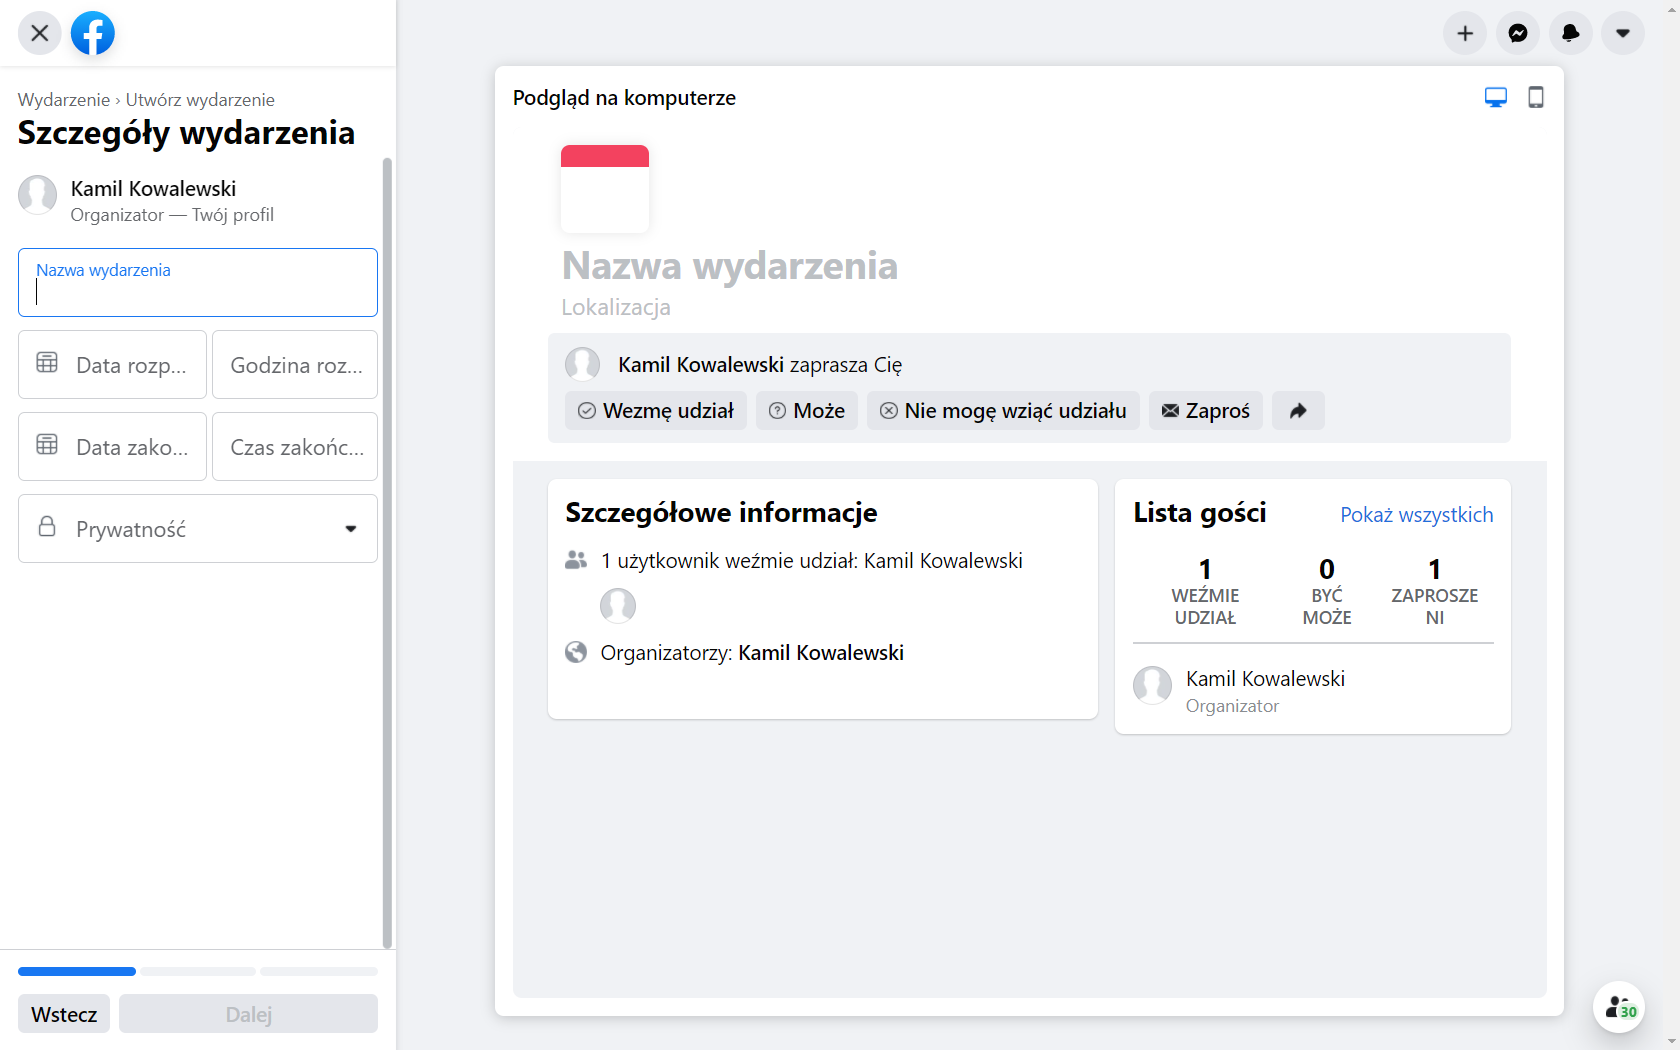
\includegraphics[width=0.7\textwidth, keepaspectratio]
            {img/chapter2/fb_event_form.png}
            \caption
            [Panel tworzenia wydarzenia na portalu Facebook]
            {Panel tworzenia wydarzenia na portalu Facebook}
            \label{chapter2:wprowadzenie_sporty:analiza_aplikacji:fb_event_form}
        \end{figure}
    }

    \section{Uzasadnienie tworzenia aplikacji \textit{Social Racetrack}}
    \label{chapter2:wprowadzenie_sporty:uzasadnienie} {
        W~związku z~widoczną luką na rynku specjalistycznych aplikacji społecznościowych
        została stworzona aplikacja \textit{Social Racetrack}. Jej głównym celem jest
        wyeliminowanie wad popularnych portali społecznościowych przedstawionych w~sekcji
        \ref{chapter2:wprowadzenie_sporty:analiza_aplikacji} oraz wypełnienie wcześniej
        wspomnianej luki. Sama aplikacja ułatwia dogodny sposób komunikacji między
        miłośnikami sportów samochodowych. Zapewnia dostęp do takich funkcji jak:
        \begin{itemize}[noitemsep,topsep=2pt]
            \item Tworzenie wydarzeń na torach wyścigowych
            \item Podpowiedzi torów
            \item Uwzględnianie przepisów bezpieczeństwa
            \item Możliwość personalizacji konta poprzez dodawanie floty pojazdów oraz
            zdobytych osiągnięć sportowych
            \item Możliwość przeglądanie kont innych użytkowników w celu poznania ich
            dorobku sportowego i~posiadanego sprzętu
            \item System łatwego dołączania do wydarzenia oraz rezygnacji z~udziału
        \end{itemize}

        \noindent Co warto wspomnieć aplikacje \textit{Social Racetrack} cechuje:
        \begin{itemize}[noitemsep,topsep=2pt]
            \item Przejrzysty i~intuicyjny interfejs użytkownika
            \item Pełna prywatność danych
            \item Brak reklam i~natrętnych komunikatów
            \item Szybkość i~płynność działania
        \end{itemize}
    }
}
\end{document}
